\section{Durchführung}
\label{sec:Durchführung}

\begin{figure}[H]
    \centering
        \centering
        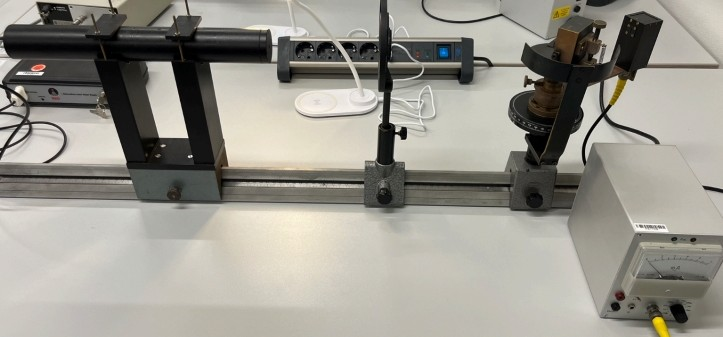
\includegraphics[width=0.7\textwidth]{Bilder/aufbau.jpg}
        \caption{Aufbau.}
    \hfill
    \label{fig:2}
\end{figure}
\noindent Gemäß \autoref{fig:2} wird das Experiment durchgeführt. Links ist
eine Hg-Hochdrucklampe zu sehen, ihr Licht wird inmitten zweier Linsen durch 
eine Spaltblende geführt. Anschließend wird das monochromatische Licht auf ein 
Geradsichtprisma gelenkt, sodass es in seine einzelnen Frequenzbereiche 
der Wellenlänge nach aufgespalten werden. Das entstehende Lichtspektrum 
wird auf eine Photozelle gerichtet, indem diese auf einem Schwenkarm 
ausgerichtet wird. Diese Vakuum-Photozelle besteht aus einem evakuiertem 
Glaskolben mit Kathode und Anode. Ersteres verfügt über eine oxidierte
Silberschicht, auf welcher Kalium aufgetragen wurde. Letzteres ist ein
Metallring über der Kathode.
\vspace{0.5em}
\\
\noindent Zwischen der Kathode und Anode wird die Gegenspannung angelegt, die 
entsprechende Apparatur dazu befindet sich unten rechts im Bild. Im Bereich 
von etwa $-1.17 \unit{\volt}$ bis $19.14 \unit{\volt}$ werden hier Spannungen 
variiert. Direkt dahinter ist das Picoamperemeter zu sehen, welches den 
Anodenstrom detektiert.

\subsection{Kennlinien der Hg-Lampe}
Für den ersten Teil des Versuches wird $U_G$ so reguliert, dass keine Elektronen 
die Anode erreichen. Sobald das der Fall ist, kann die Messung beginnen und 
die Spannung wird zunehmend in 0.005-er Schritten erhöht bis $0 \unit{\volt}$
erreicht sind. Die Spannung wird umgepolt, sodass die Elektronen nun nicht mehr 
abgebremst, sondern beschleunigt werden. $U_G$ wird weiterhin erhöht, bis sich
eine Sättigung am Amperemeter ergibt. Dann wird das Verfahren für die halbe 
Spaltbreite wiederholt. Das Ganze findet für das Spektrum des violetten Lichts 
statt.

\subsection{Planck Konstante und Austrittsarbeit}
\label{sec:aa}
Um die genannten Konstanten zu bestimmen, wird der Arm auf weitere Farbspektren 
gerichtet, diese werden dann einem Strom nahe $I = 0 \unit{\ampere}$ untersucht.
Die zu untersuchenden Spektren sind:
\vspace{0.5em}
\\
Blau: $\lambda = 435 \unit{\nano\meter}$
\vspace{0.5em}
\\
Türkis: $\lambda = 492 \unit{\nano\meter}$
\vspace{0.5em}
\\
Grün: $\lambda = 546 \unit{\nano\meter}$
\vspace{0.5em}
\\
Orange/Gelb: $\lambda = 478 \unit{\nano\meter}$
\vspace{0.5em}
\\
\noindent Für jede Messung wird ein $U$-$I$-Diagramm erstellt. Mithilfe von einer 
linearen Regression wird dann die Grenzspannung $U_G$ bestimmt. Als Funktion 
dieser gegen die Grenzspannung kann die Austrittsarbeit $W_A$ und das Planck'
sche Wirkungsquantum $h$ ermittelt werden.